\documentclass[english]{panikzettel}

\usepackage{cleveref}
\usepackage{todonotes}
\usepackage{listings,lstautogobble}
\lstset{
	language=C,
	tabsize=4,
	basicstyle=\ttfamily,
	autogobble=true,
	breaklines=true
}

\usepackage{float}
\usepackage{graphicx}

\usepackage{fontspec}
\setmonofont[
  Contextuals={Alternate},
	Scale=MatchLowercase
	]{FiraCode Nerd Font}

\newcommand{\fkt}[1]{\texttt{#1}(\(\cdot\))}

\title{Communications Systems Engineering}
\author{Moritz Hüllmann}

\begin{document}
	\maketitle
	\section{Network Programming}
	There are five socket types, but only three are relevant.
	\begin{itemize}
		\item \texttt{SOCK\_RAW}
		\item \texttt{SOCK\_STREAM}
		\item \texttt{SOCK\_DGRAM}
		\item \texttt{SOCK\_RDM}
		\item \texttt{SOCK\_SEQPACKET}
	\end{itemize}
	Combined with \textbf{Protocol Family}, communication is defined completely.
	Focus is on \textbf{IPv4/v6}.
	Relevant protocol families
	\begin{itemize}
		\item \texttt{PF\_INET} – IPv4
		\item \texttt{PF\_INET6} – IPv6
	\end{itemize}
	Sockets give access to \textbf{transport layer}.
	One may also use \texttt{AF} instead of \texttt{PF} prefixes.
	
	\subsection{C-Implemenation of Sockets}

	\begin{defi}{\fkt{socket}}
		This function creates a new reference to a socket in the OS.
		\begin{lstlisting}[language=C]
			int socket(int socket_family, int socket_type, int protocol);
		\end{lstlisting}
		\tcblower
		\texttt{protocol} – optional, if there is only one possibility. 
		Set to \texttt{0} if not wanted

		\textbf{Returns:} 0 on success, -1 on error
	\end{defi}

	\begin{defi}{\fkt{bind}}
		This socket binds a socket to a specific address and port.
		\begin{lstlisting}[language=C]
			int bind(int sock, const struct sockaddr* addr, socklen_t addrlen);
		\end{lstlisting}
		\tcblower
		\texttt{sock} – a file descriptor, i.e. the return value of \fkt{socket}

		\textbf{Returns:} 0 on success, -1 on error
	\end{defi}
	\fkt{bind} – commonly used by servers.
	\texttt{strcut sockaddr* addr} has all information regarding IPv4/v6.

	One has to be careful regarding byte order. 
	Sockets usualy require \textbf{network byte order}. 
	
	\begin{description}
		\item[\fkt{htonl}] Host to network long
		\item[\fkt{ntohl}] Network to host long
		\item[\dots] and many more
	\end{description}

	\begin{defi}{\fkt{getaddrinfo}}
		This function gets all possible based on the information passed to it.
		Can be used to determine IP addresses, ports and so on.
		\begin{lstlisting}[language=C]
			int getaddrinfo(const char *node, const char *service, const struct addrinfo *hints, struct addrinfo **res);	
		\end{lstlisting}
		\tcblower
		\texttt{hints} – used to tell the function what is should do specifically.

		\textbf{Returns:} 0 on success, -1 on error. 
		On success, \texttt{res} contains a pointer to a linked list of whatever was requested
	\end{defi}
	This function should be used everytime, one implements server/client applications, as it can handle DNS resolution, handle both IPv4 and v6 and so on.

	Suggested call order:
	\begin{enumerate}
		\item \fkt{getaddrinfo}
		\item \fkt{socket}
		\item \fkt{bind}
	\end{enumerate}

	\begin{figure}[H]
		\centering
		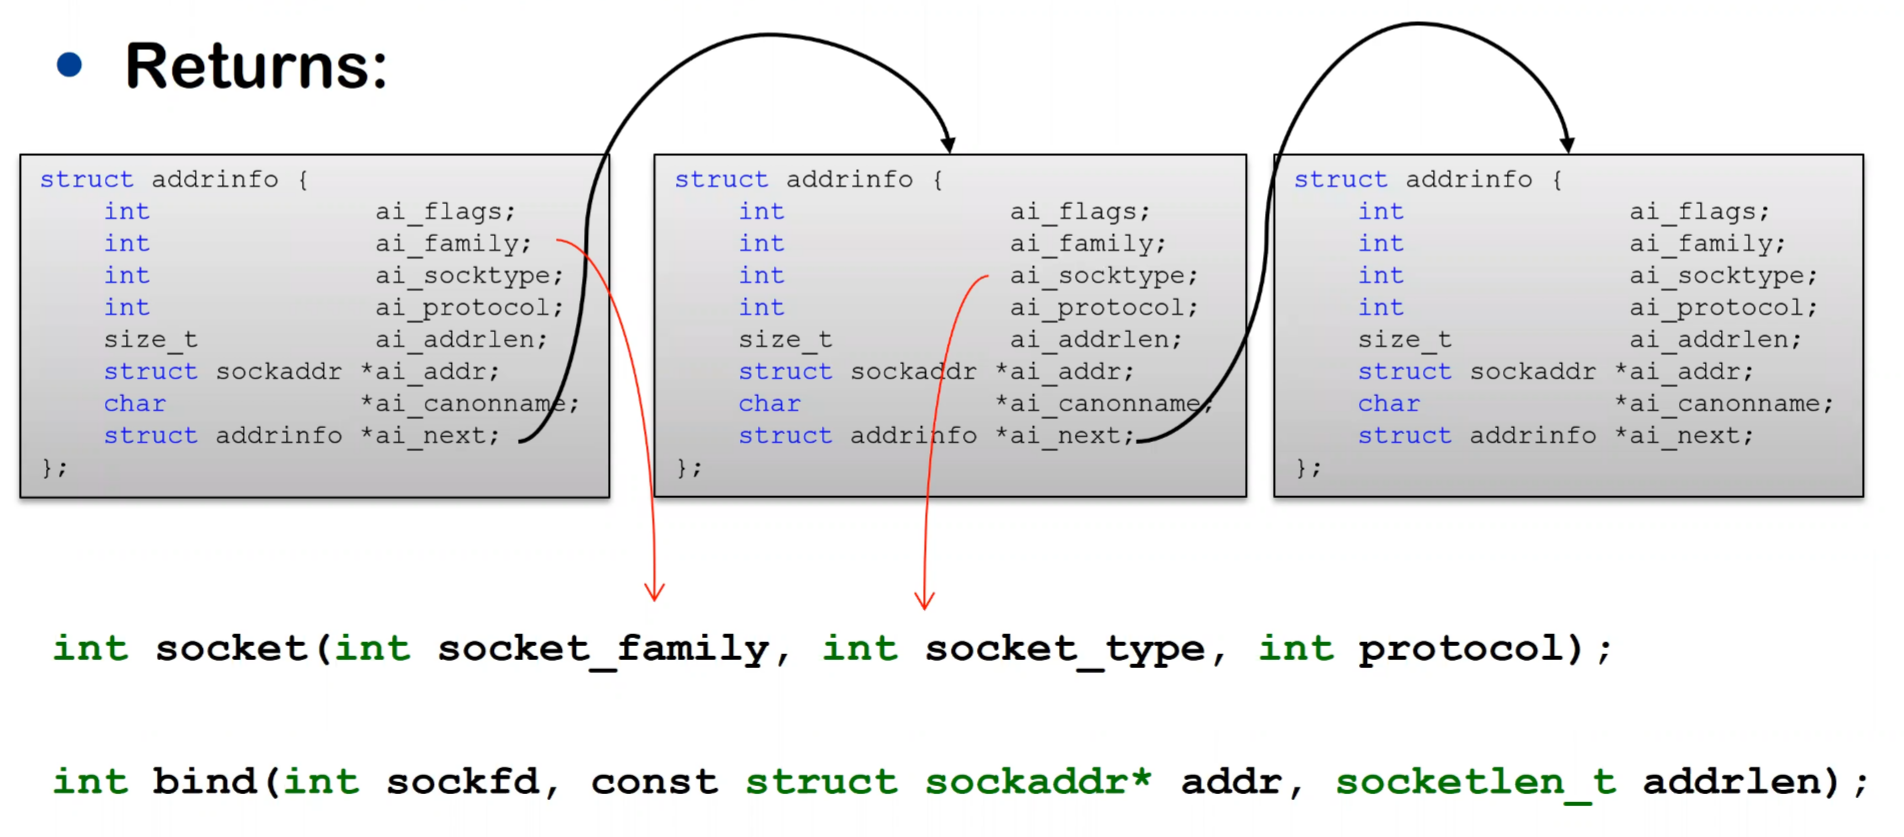
\includegraphics[width=\textwidth]{img/1-getaddrinfo-usage.png}
		\caption{How to use \fkt{getaddrinfo}. Note: All information used should originate in one block, not two as shown above.}
		\label{img-1-getaddrinfo-usage}
	\end{figure}	
	
	\subsubsection{Server-side programming}

	Up until now, only communication setup was discussed, we need to communicate now.

	\begin{defi}{\fkt{listen}}
		This functions listens for incoming connection requests.
		\begin{lstlisting}[language=C]
				int listen(int sockfd, int backlog);
		\end{lstlisting}
		\tcblower
		\texttt{sockfd} – Socket to listen on.	
		
		\texttt{backlog} – Queue length for pending requests.
	
		\textbf{Note:} This is only valid with \texttt{SOCK\_STREAM} and \texttt{SOCK\_SEQPACKET}.
	\end{defi}
	If the queue is full, the server will not answer.
	\fkt{listen} is a blocking function.

	\begin{defi}{\fkt{accept}}
		This function is used to accept requests received by \fkt{listen}.
		\begin{lstlisting}[language=C]
			int accept(int sockfd, struct sockaddr *addr, socklen_t *addrlen);
		\end{lstlisting}
		\tcblower
		\texttt{addr} – holds the address that should be accepted
		
		\texttt{addrlen} – length of \texttt{addr}. One can pass a structure that is big enough for IPv4 and IPv6.

		\textbf{Returns:} File descriptor for new socket, that handles the accepted connection from now on.
	\end{defi}

	\subsubsection{Client-side programming}

	\begin{defi}{\fkt{connect}}
		This function connects the socket to a server.
		It may perform a TCP handshake and similar things in the process.
		\begin{lstlisting}[language=C]
			int connect(int sockfd, struct sockaddr *addr, socklen_t addrlen);
		\end{lstlisting}
		\tcblower
		\texttt{addr} – address to connect to

		\texttt{addrlen} – length of the address

		\textbf{Returns:} 0 on success, -1 on failure
	\end{defi}
	
	\subsubsection{Sending and receiving}
	
	One can \textit{write} to and \textit{read} from sockets, with the following functions:
	\begin{itemize}
		\item \fkt{write} and \fkt{read}
		\item \fkt{send} and \fkt{recv} – TCP
		\item \fkt{sendto} and \fkt{recvfrom} – UDP
	\end{itemize}
	
	\begin{defi}{Stream}
		A stream is like reading from a file. TCP just decides to cut the stream at certain points and transmits each fragments as packets.
		We do not know the context of a single packet.
	\end{defi}

	\begin{defi}{Datagram}
		Messages transmitted via datagrams are not cut up by the kernel, they are send as is. If the message is too large, there either is an error, or the package gets fragmented. 
		Each datagram is self-contained, so every received packet can be seen as a unit. 
 	\end{defi}

	\begin{defi}{\fkt{send}/\fkt{write}}
		These functions can be used to write to a socket. 
		As in Linux everything is a file, one can use \fkt{write} instead of \fkt{send}.
		\begin{lstlisting}[language=C]
			ssize_t send(int sockfd, const void* buf, size_t len, int flags);
			ssize_t write(int fd, const void* buf, size_t count);
		\end{lstlisting}
		\tcblower
		\texttt{flags} – instruct kernel to handle send request in a certain way

		\texttt{buf} – Buffer with data to send

		\textbf{Returns:} Bytes actually written. -1 on error, non-negative otherwise 
		\textbf{Note:} \fkt{write} is equals to \fkt{send} with \( \texttt{flags} = 0\)
	\end{defi}

	\begin{defi}{\fkt{recv}/\fkt{read}}
		These functions are designed to read a certain amount of bytes from a socket (or file).
		\begin{lstlisting}[language=C]
			ssize_t recv(int sockfd, void* buf, size_t len, int flags);
			ssize_t read(int fd, void* buf, size_t count);
		\end{lstlisting}
		\tcblower
		Parameters are analogous to \fkt{send}.
	\end{defi}
	Actually using the return value of the reading functions is really important.
	It may be unknown, how many bytes the applications is going to receive in a single read operation.
	If \( retval \not= lenght \), then not enough was read. 

	\begin{defi}{\fkt{sendto} for connection-less sockets}
		This function sends a certain amount of bytes from a buffer to the specified address and port.
		\begin{lstlisting}[language=C]
			ssize_t sendto(int sockfd, const void* buf, size_t len, int flags, const struct sockaddr *dest_addr, socklen_t addrlen);
		\end{lstlisting}
		\tcblower
		\texttt{dest\_addr} – Address and port to send to 

		\textbf{Note:} There is no equivalent \texttt{write} function.
		
		\textbf{Note:} Parameters up to \texttt{flags} same as for \fkt{send}. 
		Exclusively for sending datagrams.
	\end{defi}

	\begin{defi}{\fkt{recvfrom} for connection-less sockets}
		This functions receives a certain amount of bytes from a given address.
		\begin{lstlisting}[language=C]
			ssize_t recvfrom(int sockfd, void* buf, size_t len, int flags, const struct sockaddr *src_addr, socklen_t *addrlen);
		\end{lstlisting}
		\tcblower
		\textbf{Note:} \texttt{src\_addr} will be replaced with the address, that really was received from. 
		\texttt{addrlen} will then hold the correct length of the structure.

		\textbf{Note:} Parameters up to \texttt{flags} same as \fkt{recv}.
	\end{defi}

	Again, if it is not known which version of IP is going to be used, use \texttt{struct sockaddr\_storage}, to allow for both versions.

	\subsubsection{Closing connections}

	There are several methods for closing a connection, each to be used in a different scenario.

	\begin{defi}{\fkt{close}}
		Drops all pakets queued for receiving and sending, and shuts down everything else related to the socket. Also frees all previously allocated space.
		\begin{lstlisting}[language=C]
			int close(int sockfd);
		\end{lstlisting}
		\tcblower
		\textbf{Returns:} 0 on success, -1 on error
	\end{defi}

	For more conservative shutdown operations, the following function can be used.

	\begin{defi}{\fkt{shutdown}}
		More conservative \fkt{close} variant.
		\begin{lstlisting}[language=C]
			int shutdown(int sockfd, int flags);
		\end{lstlisting}
		\tcblower
		\texttt{flags} – 0: no further receives, 1: no further sends, 2: both

		\textbf{Note:} Return values same as for \fkt{close}

		\textbf{Note:} Sends \texttt{FIN} and/or \texttt{FIN\_ACK}, other party might get \texttt{RST} (reset) when trying to read from the shut down socket

		\textbf{Note:} This allows all queued data to be send.
	\end{defi}

	\fkt{shutdown} cannot stand alone. 
	\fkt{close} must be called after a call to \fkt{shutdown}, as it releases all hugged \texttt{struct}s.

	\subsubsection{Connection overview}

	\begin{figure}[H]
		\centering
		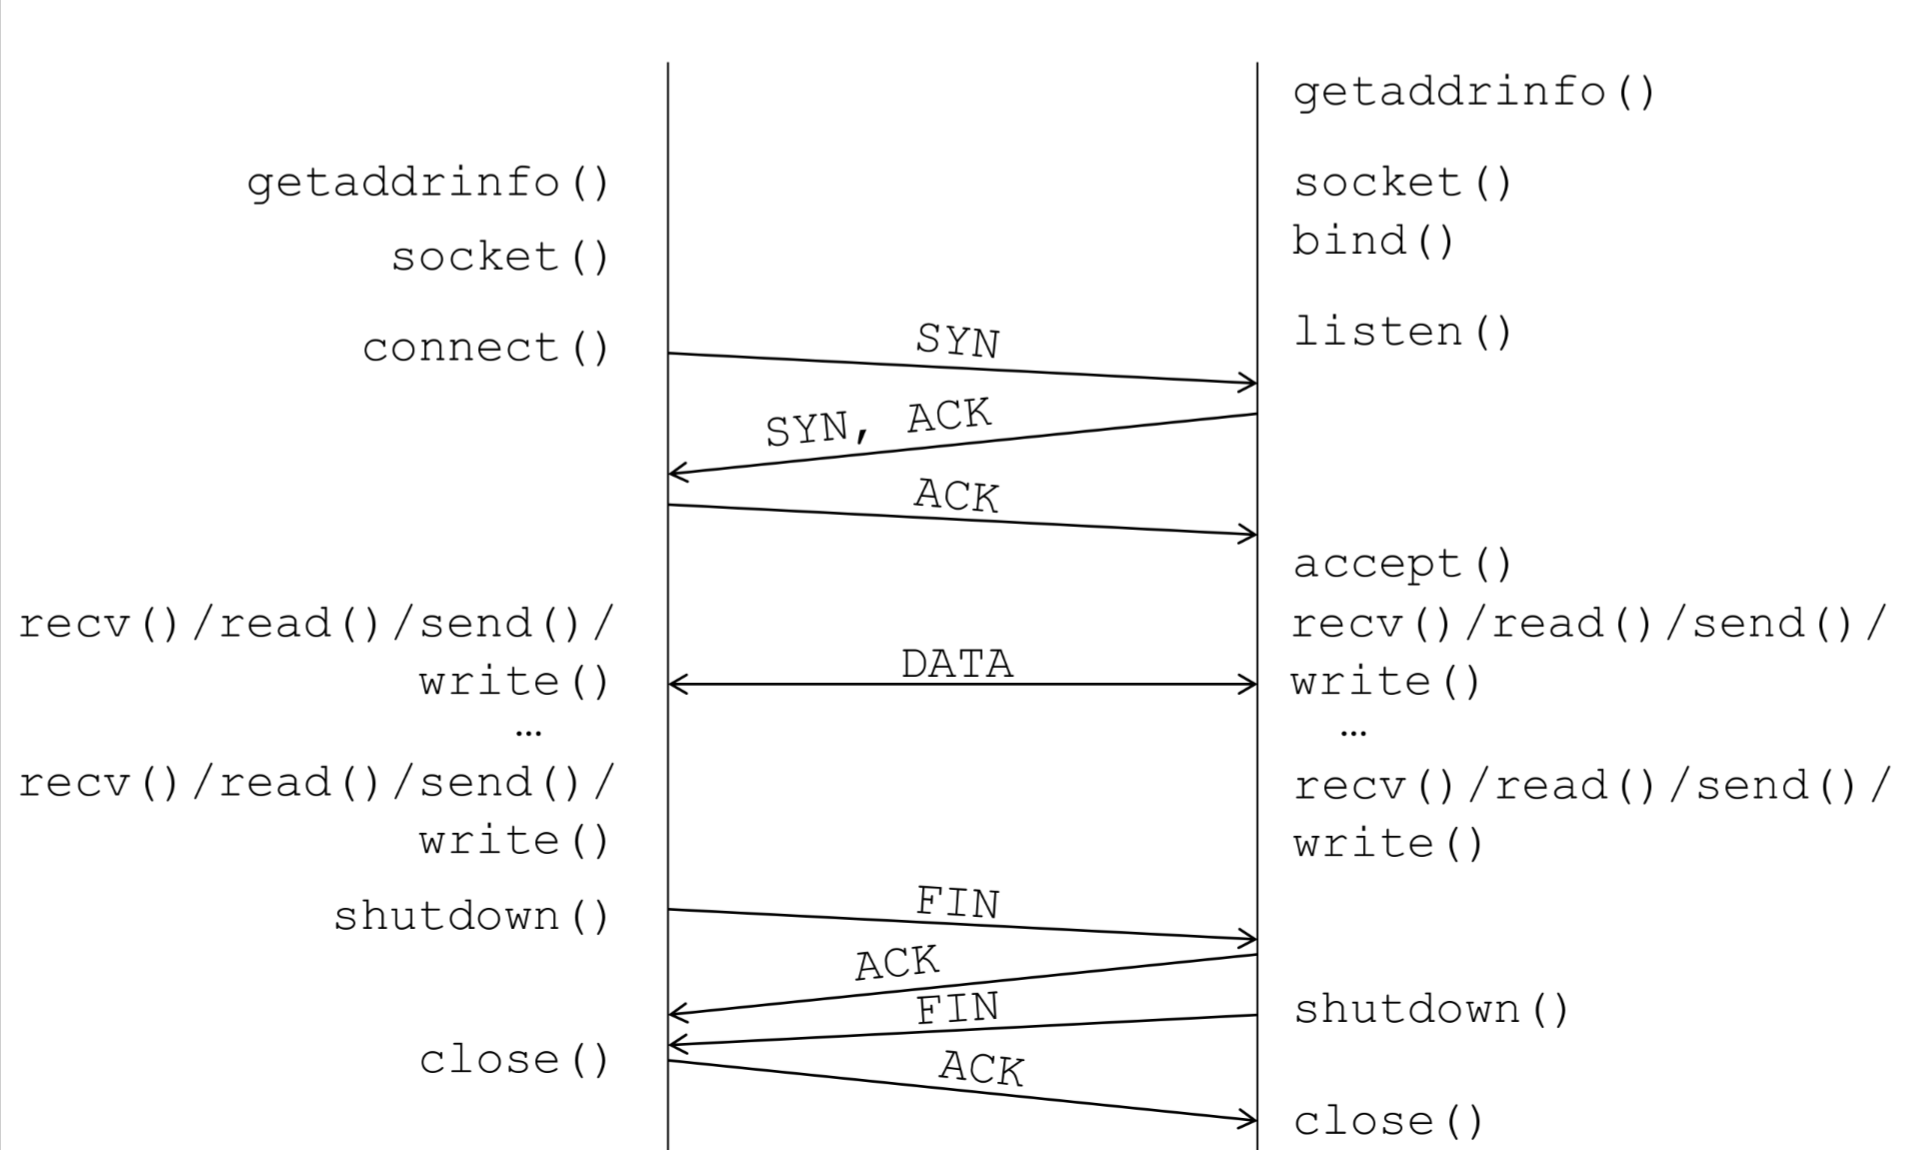
\includegraphics[width=\textwidth]{img/1-connection-overview.png}
		\caption{Overview over the course of a connection-aware socket}
		\label{img-1-connection-overview}
	\end{figure}

	\subsubsection{Configuring a socket}

	\begin{defi}{\fkt{setsockopt}}
		Apply options to sockets.
		\begin{lstlisting}[language=C]
			int setsockopt(int sockfd, int level, int optname, const void* optval, socklen_t optlen);
		\end{lstlisting}
		\tcblower
		\texttt{level} – basicalli ISO/OSI level the option should be applied to
		
		\textbf{Returns:} 0 on success, -1 on error
	\end{defi}
	
	Getting options set for a sockets uses a functions with more or less the same signature as \fkt{setsockopt}, but is called \texttt{getsockopt}.

	\texttt{I/O}-controls can also be used to set and read properties of a socket. Commonly:
	\begin{itemize}
		\item Timestamp of last received packet
		\item How many bytes are unsend (TCP)
		\item How many bytes are unread (TCP)
		\item \dots
	\end{itemize}
	
	\subsubsection{Non-blocking sockets}
	
	There are two methods that one could use: \fkt{select} and \texttt{epoll}.

	\paragraph{Non-blocking sockets using \fkt{select}}
	All network calls are blocking by default. 
	This is not optimal in a server setting, as this introduces great overhead and occupies many ressources of the server, that could be used elsewhere. 
	\textbf{Threads} are not an option for highly scalable systems, as they introduce great computation overhead.
	\fkt{fcntl} can be used to set flags to sockets, specically \texttt{O\_NONBLOCK}.
	Callbacks are called, to notify a program, if a socket is write-/readable.
	Polling is not an option, this is busy waiting.	

	\begin{defi}{\fkt{select}}
		\begin{lstlisting}[language=C]
			int select(int nfds, fd_set *readfds, fd_set *writefds, fd_set *exceptfds, struct timeval *timeout);
		\end{lstlisting}
		\tcblower
		\texttt{nfds} – highest file descriptor number in all sets + 1 
		
		\texttt{readfds} – list of sockets to monitor readability for 

		\texttt{writefds} – list of sockets to monitor writeability for

		\texttt{exceptfds} – list of sockets to monitor exceptions for
		
		\texttt{timeout} – maxium wait time
		
		\textbf{Returns:} 0 on timeout, -1 on error, else number of fd's with event \texttt{read/write/excetpfds} is then set to the sockets with events. Manual checking which sockets have events is required.
		\texttt{}
	\end{defi}

	\paragraph{Non-blocking sockets using \texttt{epoll}}

	It knows two modes:
	\begin{enumerate}
		\item level triggered, which is just as \fkt{select}
		\item and edge triggered.
	\end{enumerate}

	Edge triggered \texttt{epoll} informs on every \textit{change} of states for read and write queues, as well as excepts. 

	If there are 5 new bytes received, calling \texttt{epoll} returns that new data is readable. 
	However, if just 1 byte is read and \texttt{epoll} called again, it will block, as there is no \textbf{new} data available.

	An \texttt{epoll} file descriptor is attached to the sockets queue, directly in the kernel.
	Each \texttt{epoll} \textit{fd} has a queue of its own, and notifies for every socket listed there.

	\begin{figure}[H]
		\centering
		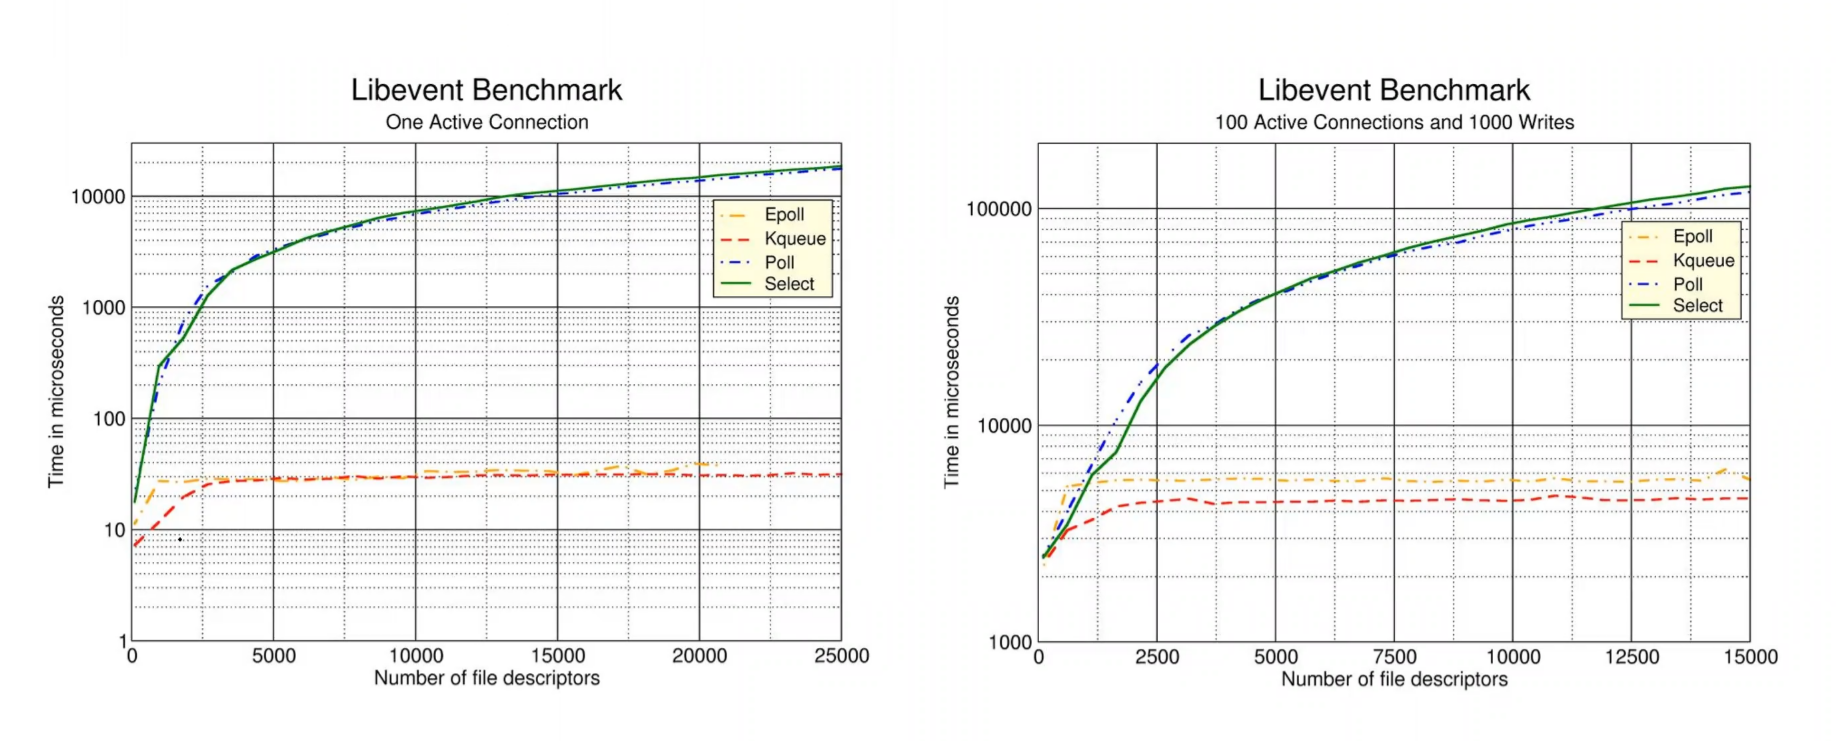
\includegraphics[width=\textwidth]{img/1-epoll-vs-select.png}
		\caption{Performance of \texttt{epoll} vs. \fkt{select}}
		\label{img-1-epoll-vs-select}
	\end{figure}

	\subsection{TCP options and packetization}
	\label{tcp-options-and-packetization}
	
	TCP needs to decide important questions: 
	\begin{enumerate}
		\item When to wait for more data from user space
		\item When to send queued data
	\end{enumerate}
	
	If not done so, every \fkt{send} results in a packet. If only one byte is send, that would result in packages with 40 bytes of overhead, but only one byte of payload.

	\subsubsection{Nagle's Algorithm}
	\label{nagles-algorithm}
	
	\begin{algo}{Nagle's Algorithm}
		This algorithm is default TCP socket behaviour.

		Small chunks are accumulated and send, when previous data was ACKed.
		\begin{lstlisting}[language=C]
			if (there is new data to send) {
				if (window size >= max(segment size) && available data >= max(segment size)) {
					complete max(segment size) and send now;
					queue remaining data;
				}
				else if (exists(data in flight waiting to be ACKed)) {
					queue data and send when ACK is received;
				}
				else {
					send data immediately;
				}
			}
		\end{lstlisting}
		\tcblower
		\textbf{Note:} This algorithm is not suited for every application, as it may wait, when an immediate send might be necessary.
	\end{algo}
	
	Disable with \texttt{TCP\_NODELAY} with \fkt{setsockopt}.

	\subsubsection{Delayed ACKs}
	\label{delayed-acks}

	Basic idea: when data is received, we will want to send data as a response.
	Piggy back ACKs for previous data on data you want to send.
	The delay is \( \leq 0.5 \textit{s} \).
	At least every second packet with MSS is ACKed immediately.
	
	This also is TCP default behaviour.
	However, don't combine with \cref{nagles-algorithm}, this may lead to unnecessary waiting times of up to 0.5 \textit{s}. 
	
	Disable with \texttt{TCP\_QUICKACK} with \fkt{setsockopt}.

	Also possible: packetize TCP yourself, using \texttt{TCP\_CORK}, which works best with \texttt{TCP\_NODELAY}.
	It will still send out MSS packets immediately.
	Allows for application level flushing.

	Can also be achieved with \fkt{send} and its \texttt{flags}, by adding \texttt{MSG\_MORE} to it.

	\subsubsection{TCP fast open}
	\label{tcp-fast-open}
	
	Normal TCP has 1 RTT delay due to 3-way handshake.

	This option adds the TCP request to TCP's \texttt{SYN} message.
	Leads to 5-7\% speed-up. 

	\textbf{Problems:}\\
	Don't process request before handshake is compelete: risk to security, if handshake would not be completed. Possible DoS scenarios:
	\begin{itemize}
		\item Resource exhaustion attack – Leave connection half open with \texttt{SYN}-flood	
		\item Reflection attack – Spoof live IP addresses, so those get spamed
	\end{itemize}
	Also problem with duplicated data. This also makes the above attacks easier.

	\textbf{Avoiding those problems:}\\
	What to do to tackle the problems
	\begin{itemize}
		\item Keep verified hosts on a \textit{secure} whitelist
		\item Only trust peers that completed a handshake – this needs a proof
		\item Application must tolerated duplicated \texttt{SYN} data
	\end{itemize}

	\begin{figure}[H]
		\centering
		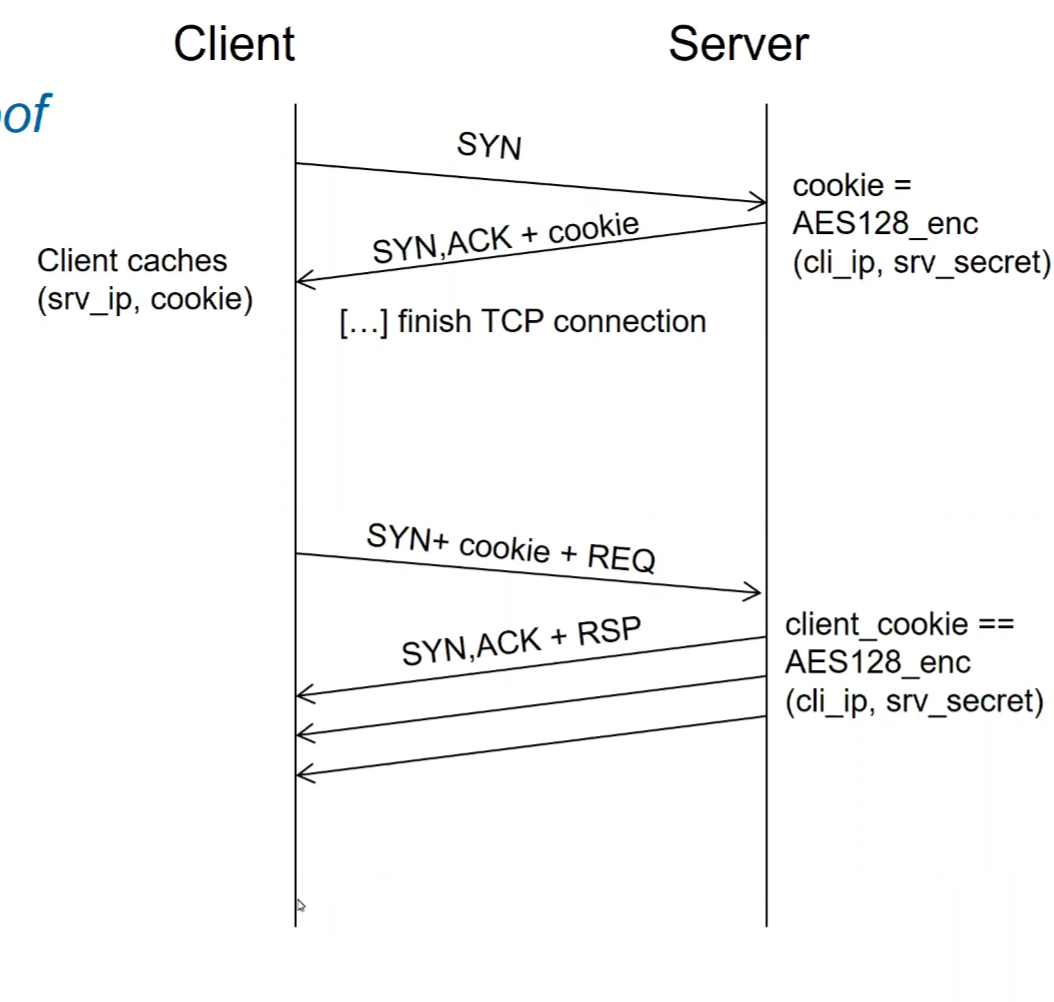
\includegraphics[width=0.65\textwidth]{img/1-tcp-fastopen-proof.png}
		\caption{Using cookie as proof of validity of connection}
		\label{img-1-tcp-fastopen-proof}
	\end{figure}

	Cookies are not valid forever. If cookie is invalid continue with normal TCP handshake.
	
	Cookies may not reach destination. 
	Can be dropped by middleboxes, also timeouts can occur.
	Cookies can be stolen \( \rightarrow \) Rediraction attacks 
	Cookies are dependent on the IP address of the client \( \rightarrow \) change in networks invalidates the cookie, so mobile usage is not optimal

	TCP fast open is not used today, as it leads to more problems than it solves.
	It also has significant problems with middleboxes.

	Activating TCP fast open on servers using \fkt{setsockopts} with \texttt{TCP\_FASTOPEN} together with a maximum count of connections.

	Activating TCP fast open for clients by piggybacking data to the connect call. 
	Also need to use \texttt{MSG\_FASTOPEN}.

	\subsubsection{Multipass TCP}
	\label{multipass-tcp}

	Enable multiple connections between clients and servers. 
	This enables for some backup paths, if one connection suddenly fails.
	However, TCP is \textit{single-path} only, meaning there can only be one connection per socket.
	This leads to poor performance for mobile users, if, for example, if you change from WiFi to 4G networks.

	How to use multi-path TCP:
	\begin{enumerate}
		\item Send options \texttt{MP\_CAPABLE} with \texttt{SYN} message to signal multi-path capability.
		\item If servers sends the same option back, both parties know, that the other party supports 
		\item Send specific \texttt{JOIN} with another \texttt{SYN} message to server, signalling to which connection to join the incoming one to.
	\end{enumerate}

	Again, there are problems with middle boxes.
	Middleboxes (esp. NAT) may \textbf{change} the following field in the IP header.
	\begin{itemize}
		\item IP source address
		\item IP destination address
		\item Source port
		\item Destination port
		\item Sequence number 
		\item ACK number
	\end{itemize}
	They especially can remove the \texttt{MP\_CAPABLE} flag, which leads to unsuccessful connection establishment \( \rightarrow \) normal TCP connection established.

	Also, non-sequential ACKs (when only looking at one path) may be dropped.
	
	Middleboxes may also change all other possible fields, but those changes are not common.
		
	\section{Design Patterns}
	\label{design-patterns}
	
	This chapter describes, how to design networking protocols properly, such that they can be extended and worked with nicely. 

	General design principles are
	\begin{itemize}
		\item Simplicity
		\item Modularity
		\item Well-foremdness
		\item Robustness
		\item Consistency
	\end{itemize}

	These lead to the 10 rules of design.

	\begin{defi}{10 rules of design}
		There are 10 rules, that every desing process regarding protocols must follow.
		\tcblower
		\begin{enumerate}
			\item Define the problem well
			\item Define the service first
			\item Design external functionality first, then internal
			\item Keep it simple
			\item Do not connect what's independent
			\item Don't impose irrelevant restrictions
			\item Build high level prototyp and validate first
			\item Implement, evaluate and \textbf{optimize} the design
			\item Check equivalence of prototyp and implementation
			\item Don't skip 1-7
		\end{enumerate}
	\end{defi}
	
	\subsection{Layering}
	\label{ss-layering}

	Layering describes a modular structure of a protocol, each layer being responsible for a distinct task.

	\begin{halfboxl}
		\textbf{Advantages}
		\begin{itemize}
			\item Smaller subproblems to handle on each layer
			\item Implementation as modules
			\item Exchangeable modules
			\item Reusable modules
		\end{itemize}
	\end{halfboxl}%	
 	\begin{halfboxr}
		\vspace{-\baselineskip}
 		\textbf{Disadvantages}
		\begin{itemize}
			\item Information is hidden \( \rightarrow \) performance loss
			\item Redundantly implemented functionality on different layers
		\end{itemize}
 	\end{halfboxr}

	\textit{Cross-layer communication} can help with redundancy, but is not common, as it is hard to change. 

\end{document}
